\documentclass[11pt]{article}
\usepackage{amsmath, amssymb}
\usepackage{geometry}
\geometry{margin=1in}
\usepackage{fancyhdr}
\usepackage{lastpage}
\usepackage{parskip} % Better paragraph spacing
\usepackage{titlesec} % Better section formatting
\usepackage{graphicx}
\usepackage{float}
\usepackage[most]{tcolorbox}
\usepackage{lmodern}
\usepackage{caption}

% Define commands for reusable content
\newcommand{\coursename}{COM-402 Information Security and Privacy}
\newcommand{\lecturenum}{05}
\newcommand{\lecturedate}{\today}
\newcommand{\professor}{Mathias Payer}

% Configure section spacing
\titlespacing*{\section}{0pt}{2ex plus 1ex minus .2ex}{1.5ex plus .2ex}
% Header / Footer
\pagestyle{fancy}
\fancyhf{}
\fancyhead[L]{\coursename}
\fancyhead[R]{Lecture \lecturenum}
\fancyfoot[L]{EPFL - Computer Science}
\fancyfoot[C]{Author: Jonathan Dutoit}
\fancyfoot[R]{Page \thepage\ of \pageref{LastPage}}

\begin{document}

\begin{center}
  {\large EPFL - Computer Science} \\[0.5em]
  {\Large \textbf{\coursename}} \\[0.5em]
  {\large Lecture \lecturenum\ --- \lecturedate} \\[0.5em]
  {\large Author: Jonathan Dutoit} \\[0.5em]
  {\large Professor: \professor} \\[0.5em]
\end{center}

\vspace{2cm}

\begin{center}
  {\LARGE \textbf{Programming Languages}}
\end{center}

\vspace{1cm}
\section*{Learning goals for today}
\begin{itemize}
	\item Understand how modern programming languages achieve key safety properties and their security implications
	\item Differentiate Type Safety, Memory Safety, and Thread Safety as policies 
	\item How to use Sandboxing and Compartmentalization to handle complex code
\end{itemize}

\vspace{0.5cm}
\begin{center}
  {\LARGE \textbf{Motivation}}
\end{center}

\vspace{0.3cm}

\section*{Google "Two out of Three" Security Rule}

Developer may only select 2 of 3 options 

Using a "safe" programming languages makes 2-out-of-3 rule unnecessary 

% Quick centered image
\begin{figure}[H]
    \centering
    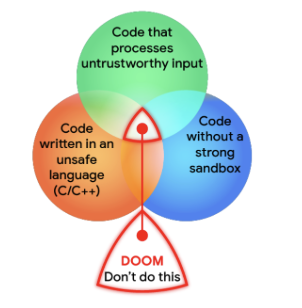
\includegraphics[width=0.4\textwidth]{2-out-of-3}
    \label{fig:LABEL}
\end{figure}

\section*{Consequences of Memory Safety Vulnerabilities}

Memory safety issue  means that an attacker can modify your memory. If you think about the process that is executing code (load, compute, store machine), thus the attacker has the power to modify the memory and make your program do arbitrary things. Memory safety issues are \textbf{really \textcolor{red}{severe}}. 

In 2022, memory-safety issues composed 86\% of critical severity security vulnerabilities, highest ranking. 

\textbf{Memory safety violations are most common:}A major portion (224/1228 $\sim$ 18\%) of bugs found by SyzBot is still memory corruption errors in Linux Kernel. 

\section*{Memory Safety}

% Quick centered image
\begin{figure}[H]
    \centering
    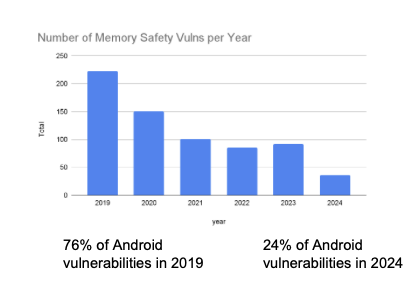
\includegraphics[width=0.6\textwidth]{memory-safety}
    \label{fig:LABEL}
\end{figure}

\begin{itemize}
	\item ~70\% of Android's high severity security vulnerabilities (2021)
	\item Android 13 is first Android release where majority of new code is in a memory safe language
\end{itemize}


\textbf{Most bugs are in new code}: that's why replacing legacy code with their new Rust implementation then just implies we're just going to have much more bugs in Rust. Replacing legacy issues is not the solution. Rust may be a safe language and thus implying no memory vulnerabilities, but rewriting code is complex.

\textbf{Is a Safe Language Better for Security?}

"[The] NSA recommends using a memory safe language when possible. While the use of added protections to non memory safe languages and the use of memory safe languages do not provide absolute protection against exploitable memory issues, they do provide considerable protection.”

A safe programming language leaves you more time to handle programming logic than memory or handling other operations aspects. 

\textbf{Three Types of Safety}:

\begin{itemize}
	\item Type Safety
	\item Memory Safety
	\item Thread Safety
\end{itemize}

\newpage
\begin{center}
  {\LARGE \textbf{Type Safety}} \\
  Is the object an elephant or a crocodile?
\end{center}

\vspace{0.5cm}

\section*{Type System}

\textit{Logical system that assigns a \textbf{type} to every \textbf{term} (variable, expression, function)}

Type of a \textbf{value} specifies which operations can be applied to it

Type of a \textbf{variable} limits values that it can be assigned

Type of an \textbf{expression/function} delimits values it accepts and can produce

Many different type systems
\begin{itemize}
	\item Static/dynamic
	\item Declared/inferred
	\item Strict/relaxed
\end{itemize}

\textit{Well-typed programs cannot "go wrong"}. (Robin Milner)

If a type system is sound, then expressions accepted by that type system must evaluate to a value of the appropriate type (rather than produce a value of some other, unrelated type or crash with a type error). A language is type-safe if the only operations that can be performed on data in the language are those sanctioned by the type of the data.

\begin{itemize}
	\item Type safety depends on the language
	\item Influenced by static/dynamic semantics
\end{itemize}

\section*{Static/Dynamic Typing}

\textbf{Static} type system is checked by the compiler (or preprocessors) before program executes
\begin{itemize}
	\item Type checker uses typing rules to determine type of all terms
	\item Compare inferred types against declared types and operations performed on values
	\item Mismatch is typing error
\end{itemize}

\textbf{Dynamic} type system tracks types of objects at runtime and prevents improper operations from being applied to them.

\section*{Typing Pros/Cons}

\textbf{Static} -- checked at compile time
\begin{itemize}
	\item No runtime overhead (memory or time)
	\item Find errors before program runs
	\item Find all errors
	\item Better for building reliable systems and groups of developers
\end{itemize}

\textbf{Dynamic} -- checked at runtime
\begin{itemize}
	\item More flexible (at least without complex type system)
	\item Fewer type declarations
	\item Better for quick and dirty programming ("scripting")
\end{itemize}

\section*{Declared/Inferred Types}

Languages previously required full type declarations for all functions and variables. Compilers only infer expression types.

Hindley-Milner type inference (Algorithm W) used in Haskell. 
Later spread to other languages.

\begin{itemize}
	\item Declare function argument and result type
	\item Compiler infers types in function body
	\item Scala, C#, Java (v8), Typescript, ...
\end{itemize}
% Quick centered image
\begin{figure}[H]
    \centering
    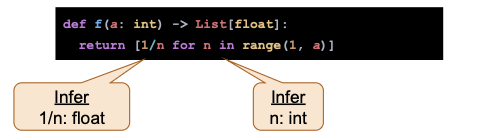
\includegraphics[width=0.7\textwidth]{declared-inferred}
    \label{fig:LABEL}
\end{figure}

\section*{Strict/Relaxed (or Weak)}

C is not strict! It "trusts" programmer-supplied type conversions.

% Quick centered image
\begin{figure}[H]
    \centering
    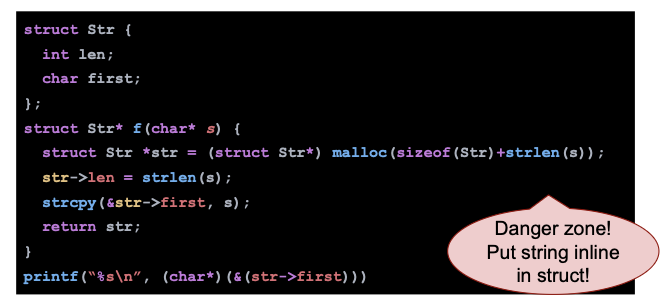
\includegraphics[width=0.8\textwidth]{weak}
    \label{fig:LABEL}
\end{figure}

\section*{What's Up with C's Type System?}

C was a thin layer over assembly language, designed by talented programmer for talented programmer 

\begin{itemize}
	\item Machines were slow. Memory was tight
\end{itemize}

Type system did not constrain programmer or prevent them from using assembly language tricks

Clearly successful, but times change
\begin{itemize}
	\item Correctness and security are far more important, and C's type system it not helpful
\end{itemize}

\section*{Type Safety and Security}

Type checking is the only "automatic" bug detection technique in widespread use
\begin{itemize}
	\item Type system might prevent you from expressing something exactly in the manner you want
	\item But it will not stop you from expressing a computation: \\
	Language with type system is still Turing-complete
	\item Problems found by sound type system are real errors: No false positives
\end{itemize}

Bugs do not always cause security problems, but they can

Type system can enforce rules that enhance security

\vspace{0.5cm}
\begin{center}
  {\LARGE \textbf{Memory Safety}} \\
  Is the monkey caged or free?
\end{center}

\vspace{0.5cm}

\section*{Memory Safety}

Memory safety is an essential programming language property

Code can only access data within live regions of memory whose pointer is properly obtained
% Quick centered image
\begin{figure}[H]
    \centering
    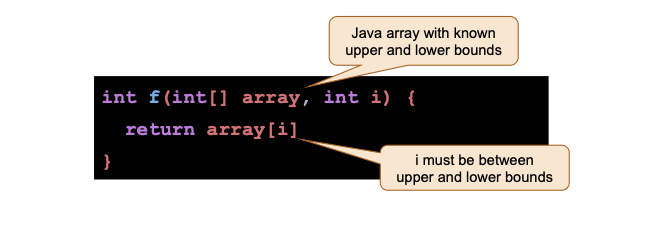
\includegraphics[width=0.8\textwidth]{memory-safety-java}
    \label{fig:LABEL}
\end{figure}

\textit{Memory safety ensures that only valid objects are accessed in bounds}

\textbf{Spatial memory safety}: objects are only accessed in bounds
\begin{itemize}
	\item After pointer arithmetic, the new pointer still points to the same object
\end{itemize}

\textbf{Temporal memory safety}: only valid objects are accessed
\begin{itemize}
	\item The underlying object has not been freed
\end{itemize}

\section*{Memory Corruption}

Unintended modification of memory location due to missing / faulty safety check

% Quick centered image
\begin{figure}[H]
    \centering
    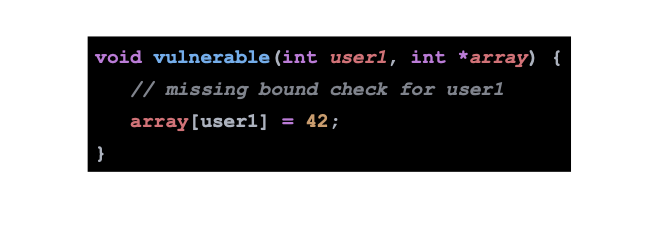
\includegraphics[width=0.8\textwidth]{memory-corrup}
    \label{fig:LABEL}
\end{figure}

\section*{Spatial Memory Safety Error}

The pointer is updated to point outside of the valid object

The pointer is used to dereference invalid memory

% Quick centered image
\begin{figure}[H]
    \centering
    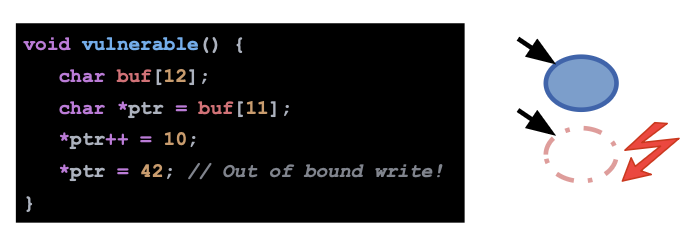
\includegraphics[width=0.7\textwidth]{spatial-memory}
    \label{fig:LABEL}
\end{figure}

\section*{Temporal Memory Safety Error}

The referenced object is freed and no longer "live". The pointer is used to dereference invalid memory. "Use after free"

\section*{Memory Safety: Implementation}

Bounds checking
\begin{itemize}
	\item Check that every indexed memory reference is within array bounds
	\item Compiler optimizations can eliminate some runtime checks
\end{itemize}

Lifetime tracking
\begin{itemize}
	\item Use after free is prohibited (e.g., by trapping accesses)
	\item Double free is prohibited (e.g., by delaying frees)
	\item Memory leakage is bad (but allowed)
\end{itemize}
Automated storage reclamation
\begin{itemize}
	\item Garbage collection
	\item Reference counting
	\item Smart pointers/borrow checking
\end{itemize}

\section*{Spatial Memory Safety: Array Access}

Every region of memory has a length associated with it
\begin{itemize}
	\item C's interior pointers make tracking more complex
	\item Programmer needs to verify that every memory access is in-bounds manually
	\item Almost every other modern PL automatically inserts bound check for array access
\end{itemize}
% Quick centered image
\begin{figure}[H]
    \centering
    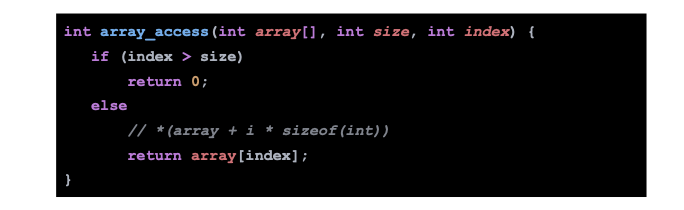
\includegraphics[width=0.8\textwidth]{array-access}
    \label{fig:LABEL}
\end{figure}

\section*{Rust Bounds Checking}

% Quick centered image
\begin{figure}[H]
    \centering
    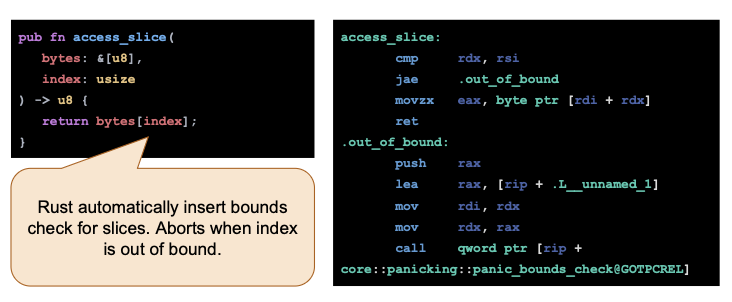
\includegraphics[width=1\textwidth]{rust}
    \label{fig:LABEL}
\end{figure}

\section*{Overhead of Bounds Checking}

Overhead for enforcing spatial memory safety for C code is significant
\begin{itemize}
	\item Softbound reporter 67\% overhead
	\item Unfortunately, C's arbitrary pointer arithmetic, conflation of pointers and arrays, and programmer-visible memory layout make retrofitting C/C++ with spatial safety guarantees extremely challenging.
\end{itemize}

Overhead for Java is not nearly as large
\begin{itemize}
	\item 3-10\% on small benchamarks
	\item found roughly the same for Rust
\end{itemize}

\section*{Automated Storage Reclamation}

Reclaim and reuse memory that will not be accessed in future execution
\begin{itemize}
	\item Conservative approximation: reclaim when memory is not reachable
\end{itemize}

Prevent errors with manual reclamation (malloc/free)

\begin{itemize}
	\item Double free
	\item Use after free
	\item (not freeing)
\end{itemize}

Many algorithms (!)
\begin{itemize}
	\item Reference counting
	\item Garbage collection
\end{itemize}

\section*{Temporal Memory Safety and Security}

\textbf{Cool lab/project}: implementing my own memory allocator (managing heap) 

Double free is an \textbf{integrity} concern
\begin{itemize}
	\item libc's memory allocator stores \textbf{metadata} alongside allocated objects.
	\item Freeing memory chunks twice will \textbf{corrupt} these metadata.
	\item The corrupted metadata can lead to two different pointers pointing to the same memory location. If an attacker controls one of those pointers, they can change the contents of that memory, which can cause security issues or even allow them to execute code.
\end{itemize}
Missing free is an \textbf{availability} concern
\begin{itemize}
	\item Basis for denial-of-service attacks (Out-of-Memory)
\end{itemize}

\section*{Reference Counting}

Every block of memory maintains a count of numbers of pointers to it
\begin{itemize}
	\item One when block allocated
	\item Copying pointer increments count
	\item Dropping pointer decrements count
\end{itemize}

Conceptually simple, but fidgety to get right (try it)

Memory freed immediately when last pointer is dropped (count = 0)

\begin{itemize}
	\item No pauses (unlinke Garbage Collection)
	\item Incr/Decr overhead can be significant
\end{itemize}

Count never reaches zero in graphs with cycles. 

Language implementations: Python, PHP

\section*{Garbage Collection (GC)}

When program is running out of free memory, stop and run collector to find unreachable objects

Pauses program execution

Uncollected garbage increases memory requirements

May be less expensive than RC

Collects unreachable cycle structures

Language implementations: JavaScript (v8, SpiderMonkey), Ruby, Lua

\textbf{Most common implementation of GC}: \textit{Mark and Sweep}, made with a \verb|Root Set| and marking objects that have memory references, and sweeping all that don't in the second phase. 

\section*{GC overhead}

Garbage collection overhead is difficult to measure
\begin{itemize}
	\item What is baseline? No allocation? Malloc/free? Other GC?
	\item GC affects behaviour of caches and program performance
\end{itemize}

Has a reputation for being significant
\begin{itemize}
	\item Depends on how program is written as well
\end{itemize}

Most troublesome is unpredictable interruptions
\begin{itemize}
	\item There are pause-free GCs
\end{itemize}

\section*{C++ Smart Pointers}

AS a intermediary step, C++ introduced the notion of "Smart Pointers", for automatic memory management. (Note: not mandatory to use them.)

Smart pointers automatically free their referenced content when it goes out of scope (or refcount reaches 0)

% Quick centered image
\begin{figure}[H]
    \centering
    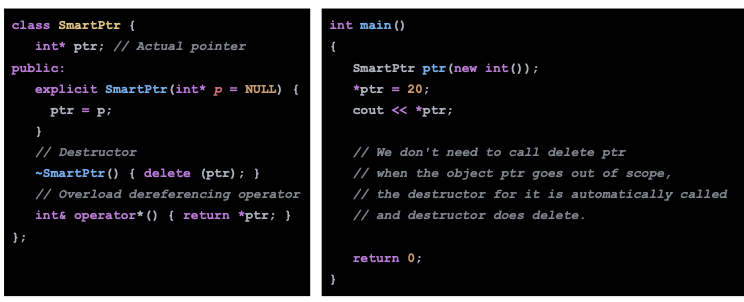
\includegraphics[width=0.8\textwidth]{smart-pointers}
    \label{fig:LABEL}
\end{figure}

\section*{Rust}
Safe programming language (type and memory). Meant for low-end and operating systems as an alternative for C or low-level languages.
\begin{itemize}
	\item Ownership types reduce need for runtime garbage collection
	\item Allows unsafe code
\end{itemize}

For low-level programming
\begin{itemize}
	\item Efficient code, no garbage collection, optional reference counting
\end{itemize}
Becoming popular for systems programming
\begin{itemize}
	\item Already in use for Linux kernel modules
\end{itemize}

\section*{Rust Ownership}

Variables \textbf{own} the value they are bound to (contain)

When variable goes out of scope, value is deallocated

Key restriction: exactly \textbf{one} variable can be bound to a value

A step forward from C++ smart pointers, as the compiler strictly enforces the constraint. In C++, developers can still choose to use raw pointers.
% Quick centered image
\begin{figure}[H]
    \centering
    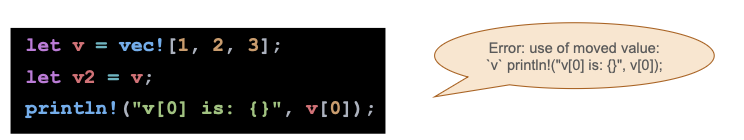
\includegraphics[width=0.8\textwidth]{own}
    \label{fig:LABEL}
\end{figure}

\section*{Rust "Borrowing"}

Ownership is very restrictive rule that often gets in the way
\begin{itemize}
	\item How do we pass a value to a function?
\end{itemize}

"Borrowing" handles common situations by sharing ownership between two variables so long as
\begin{itemize}
	\item Borrower's lifetime is no longer than owner's lifetime
	\item Either one writer or multiple readers
\end{itemize}

% Quick centered image
\begin{figure}[H]
    \centering
    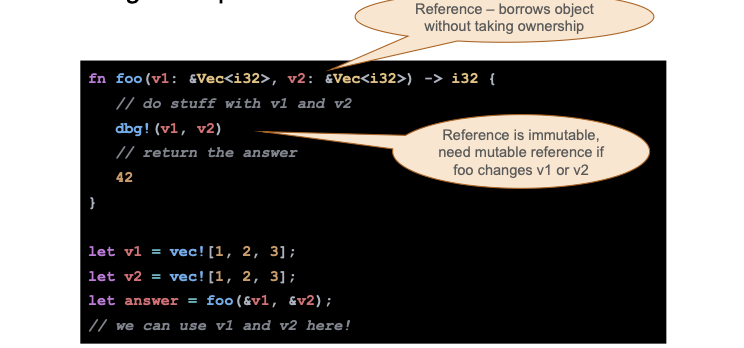
\includegraphics[width=0.8\textwidth]{borrow}
    \label{fig:LABEL}
\end{figure}

\textbf{Cannot have mutable and immutable borrow to a value at the same time}

\section*{Rust Ownership Pain}

"Implemented a linked list" is a meme in the Rust community. 

\begin{itemize}
	\item People wrote an 8-chapter book on implementing linked lists in Rust.
	\item A singly linked list is already quite verbose. Need to use \verb|Option| and \verb|Box| 
	\item A doubly linked is challenging due to cyclic reference of the previous node and next node.
\end{itemize}

\section*{Unsafe Code}

Rust also allows unsafe code that would not pass borrow checker

Put unsafe code in module and wrap in safe interface

Almost all non-trivial data structures implemented this way
\begin{itemize}
	\item Linked lists, Trees
	\item What does that say about type system?
\end{itemize}

Easier to understand and hand-verify a small amount of code that is explicitly marked unsafe

\section*{Rewrite Everything in Rust?}
In many cases, simply not possible
\begin{itemize}
	\item Chromium core is over 33 million lines of code. (Mostly C++)
	\item The Linux kernel is around 30 million lines of code (Mostly C)
	\item Simply too much to rewrite
\end{itemize}

For old code
\begin{itemize}
	\item Employ fuzzing, mitigation and hardening (Defense in-depth)
\end{itemize}

For newer code
\begin{itemize}
	\item Prefer safe language like Rust (Linux kernel modules, Android binder have been rewritten or new code is not Rust)
\end{itemize}
Clean state not needed, simply writing new code in Rust suffices!

\vspace{0.5cm}
\begin{center}
  {\LARGE \textbf{Thread Safety}} \\
  Code runs in parallel and may access the same data structures faster (or slower)
\end{center}

\vspace{0.5cm}

\section*{Thread Safety}

\textit{Thread-safe code only manipulates shared data structures in a manner that ensures that all threads behave properly and fulfill their design specifications without unintended interaction.}

Examples of concurrency bugs
\begin{itemize}
	\item Race Condition: When two or more threads attempt to access and modify shared data simultaneously without proper synchronization, it can lead to inconsistent data states.
	\item Deadlock: Deadlocks occur when two or more threads are blocked forever, each waiting for the other to release a resource.

\end{itemize}

\section*{Dirty CoW}

A local \textbf{privilege escalation} attack that exploits a \textbf{race condition} in the Linux Kernel memory-management subsystem.

CoW: Copy on Write, a mechanism for efficiently sharing modifiable data. Used extensively in the \verb|mmap| and \verb|fork| syscall.

With the right timing, a read-only mapping of a file can be turned into a writable mapping.

\section*{Thread Safety in Programming Languages}

Modern languages include type-safe synchronization primitives in their standard lib: 
\begin{itemize}
	\item Locks
	\item Semaphores
	\item Atomic Variables, ...
\end{itemize}

Other thread-safe language constructs
\begin{itemize}
	\item Java: \verb|synchronized| keyword
	\item Go: goroutines and channels
	\item Rust: owernership
\end{itemize}

Modern languages makes it easier to write thread-safe program, but ultimately it’s the programmer’s responsibility to ensure the correctness of concurrent programs.

\section*{Thread Safety in Java}

In java, the \verb|synchronized| keyword is used in the declaration of a method or code block to acquire the mutex lock for an object while the current thread executes the code.

% Quick centered image
\begin{figure}[H]
    \centering
    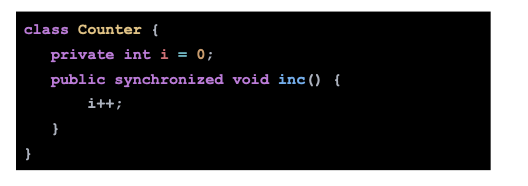
\includegraphics[width=0.8\textwidth]{synchro}
    \label{fig:LABEL}
\end{figure}

\section*{Thread Safety in Go}

\textit{Don't communicate by sharing memory, share memory by communicating}

\textbf{Goroutines}: threads created by the go runtime, cheap and fast.

\textbf{Channels}: means of communication between goroutines. Data is \textbf{copied} from one end of the channel to another.

It's possible to send pointers, but that once again may create issues.

\section*{Thread Safety in Rust}

The same mechanism that guarantees temporal memory safety also ensures thread safety: Ownership

Recall in Rust borrowing:
\begin{itemize}
	\item Owner's lifetime must outlast borrowers lifetime $\Rightarrow$ No use-after-free
	\item Either one write or multiple readers $\Rightarrow$ no data races
\end{itemize}

If you violate this, you get a \textbf{compilation error!}

\vspace{0.5cm}
\begin{center}
	{\LARGE \textbf{Sandboxing & Compartmentalization}}
\end{center}

\vspace{0.5cm}

\section*{Principle of Least Privilege}

\textbf{The principle of least privilege ensures that a component has the least privileges needed to function}

\begin{itemize}
	\item No extra functionality is present
	\item Any additionally removed functionality would impact (some) functionality 
	\item Any added functionality would not increase (any) functionality 
\end{itemize}

\section*{Sandboxing}

Sandboxing implements \textit{principle of least privilege} by running programs (often untrusted code) in an isolated, restricted environment

Sandboxing is usually a implementation feature of programming languages instead of design feature. Depending on the context/application, a script may or may not be sandboxed. 

Implemented by restricting access to certain library/system calls

\begin{itemize}
	\item \verb|secomp| (SeLinux)
	\item \verb|cgroup| (Docker)
	\item \verb|rlbox| (Firefox)
\end{itemize}

Implementation "only" at the language level is challenging
\section*{Sandboxing Example}

JavaScript/Web Assembly inside the browser

Without explicit permission from the user, opening a web page or document shouldn't leak secrets in your local hard disk.

The premise of sandboxing providing security relies entirely on the implementation of the sandbox. Bugs may still lead to sandbox breaches. 


\section*{Sandboxing: Hard to Get Right}

Flash and VBA macros used to be security nightmares (now phased out)

JavaScript engine bugs remain a source of critical browser vulnerabilities.

\section*{Compartimentalization}

Compartmentalization can enforce \textbf{principle of least privilege}

Break a complex system into small components

Limit the access of entities to only what is necessary

Prevent error propagation in the system to diminish impact

\section*{Compartmentalization: Chromium}

\textbf{Sandboxed render engines}: cannot affect the world, except via the exposed API
\begin{itemize}
	\item Start process, establish IPC channel
	\item Drop all access privileges
	\item Do not require admin rights
\end{itemize}

If a webpage in a tab crashes, it should not bring other tabs or the entire browser down!

\textbf{Browser kernel API}: decide how render engines influence the outside world

\begin{itemize}
	\item User interaction: display rendered bitmaps, forward input events
	\item Storage: manage cookies, passwords, authorize uploads, restrict downloads
	\item Network: handle HTTP requests and responses, restrict certain schemes (e.g., file://) 
\end{itemize}

\section*{Compartmentalization in PL}

\begin{itemize}
	\item What should a basic entity be: functions, libraries? (component)
	\item How should each component interact with each other? (policy) 
\end{itemize}

\section*{Summary}

Memory safety issues remain dominant. Modern PLs achieve memory safety through bounds checking, lifetime tracking and automatic storage reclamation. 

A programming language's type system can be static/dynamic, inferred/declared, strict/relaxed. A well-designed type system prevents type confusion bugs.

Modern languages provide synchronization primitives and incorporate thread-safe constructs in their design

Sandboxing/compartmentalization can enforce least privileges.
\end{document}
